This section covers basic performance tests, i.e. how specific algorithms scale in parallel with increasing \emph{number of processors}. So far, all calculations for this research were conducted on the Lichtenberg high performance computer of the TU Darmstadt

\section{Parallel Efficiency - Navier-Stokes problems}
Different solver strategies are conducted to solve the fully coupled incompressible Navier-Stokes equations. At the moment the following strategies can be examined:
\begin{itemize}
	\item Linearizsation of the NSE with: Newton(Gmres) or Picard
	\item Solving the linear problem with a Gmres approach
	\item Preconditioning with Additive-Schwarz domain decomposition (with coarse solve on the coarsest multigrid level) and direct solver MUMPS for the Blocks
\end{itemize}
\subsection{Simple 3D sphere immersed in a fluid flow}
\label{sec:MPIPerformanceSphere}
The problem
\begin{equation}
\left\{ \begin{array} {rclll}
\rho_f\Big(\frac{\partial \vec{u}}{\partial t}+ \vec{u} \cdot \nabla \vec{u}\Big) +\nabla p - \mu_f \Delta \vec{u} & = & \vec{f}                   
& \text{and}\   &  \\
% ----
\nabla \cdot \vec{u} & = & 0                             
& \text{in}\ \Omega = (-5,10) \times (-5,5) \times (-5,5)  & \\
 \vec{u}_D & = & 0                             
& \text{on}\ \Gamma_D = \{ (x,y,z,t) \in \real^3; \ z = -5,5 \} 
& \text{Dirichlet-boundary}\\
 \vec{u}_S & = & 0                             
 & \text{on}\ \Gamma_S = \{ (x,y,z) \in \real^3; \ x^2+y^2+z^2 = 1 \}
& \text{Dirichlet-boundary} \\
 p_O & = & 0                             
& \text{on}\ \Gamma_O = \{ (x,y,z) \in \real^3; \ x = 10 \}
& \text{Dirichlet-boundary} \\
% ----
\vec{u}(x,-5,z) & = & \vec{u}(x,5,z)  
& \text{on}\ \Gamma_P = \partial \Omega \setminus \Gamma_D \setminus \Gamma_S \setminus \Gamma_O
& \text{Periodic-boundary}\\
\vec{u}_0(x,y,z) & = & \{1,0,0\}  
& \text{in}\ \Omega = (-5,10) \times (-5,5) \times (-5,5)   
& \text{Initial Condition}
\end{array} \right.
\label{eq:NavierStokesSphereBenchmark}
\end{equation}
is investigated on a 64x16x16 cell Cartesian grid. The physical parameters of the fluid are 
choosen to be $\rho_f=1$ and $\mu_f=0.002$ which renders down to a Reynolds Number of 100. 
The problem basically describes a sphere flow between two plates.

\graphicspath{{./apdx-MPISolverPerformance/strongScaling/NSESphere/plots/}}

\begin{figure}[h!]
	\begin{center}
		% GNUPLOT: LaTeX picture with Postscript
\begingroup
  \makeatletter
  \providecommand\color[2][]{%
    \GenericError{(gnuplot) \space\space\space\@spaces}{%
      Package color not loaded in conjunction with
      terminal option `colourtext'%
    }{See the gnuplot documentation for explanation.%
    }{Either use 'blacktext' in gnuplot or load the package
      color.sty in LaTeX.}%
    \renewcommand\color[2][]{}%
  }%
  \providecommand\includegraphics[2][]{%
    \GenericError{(gnuplot) \space\space\space\@spaces}{%
      Package graphicx or graphics not loaded%
    }{See the gnuplot documentation for explanation.%
    }{The gnuplot epslatex terminal needs graphicx.sty or graphics.sty.}%
    \renewcommand\includegraphics[2][]{}%
  }%
  \providecommand\rotatebox[2]{#2}%
  \@ifundefined{ifGPcolor}{%
    \newif\ifGPcolor
    \GPcolortrue
  }{}%
  \@ifundefined{ifGPblacktext}{%
    \newif\ifGPblacktext
    \GPblacktexttrue
  }{}%
  % define a \g@addto@macro without @ in the name:
  \let\gplgaddtomacro\g@addto@macro
  % define empty templates for all commands taking text:
  \gdef\gplbacktext{}%
  \gdef\gplfronttext{}%
  \makeatother
  \ifGPblacktext
    % no textcolor at all
    \def\colorrgb#1{}%
    \def\colorgray#1{}%
  \else
    % gray or color?
    \ifGPcolor
      \def\colorrgb#1{\color[rgb]{#1}}%
      \def\colorgray#1{\color[gray]{#1}}%
      \expandafter\def\csname LTw\endcsname{\color{white}}%
      \expandafter\def\csname LTb\endcsname{\color{black}}%
      \expandafter\def\csname LTa\endcsname{\color{black}}%
      \expandafter\def\csname LT0\endcsname{\color[rgb]{1,0,0}}%
      \expandafter\def\csname LT1\endcsname{\color[rgb]{0,1,0}}%
      \expandafter\def\csname LT2\endcsname{\color[rgb]{0,0,1}}%
      \expandafter\def\csname LT3\endcsname{\color[rgb]{1,0,1}}%
      \expandafter\def\csname LT4\endcsname{\color[rgb]{0,1,1}}%
      \expandafter\def\csname LT5\endcsname{\color[rgb]{1,1,0}}%
      \expandafter\def\csname LT6\endcsname{\color[rgb]{0,0,0}}%
      \expandafter\def\csname LT7\endcsname{\color[rgb]{1,0.3,0}}%
      \expandafter\def\csname LT8\endcsname{\color[rgb]{0.5,0.5,0.5}}%
    \else
      % gray
      \def\colorrgb#1{\color{black}}%
      \def\colorgray#1{\color[gray]{#1}}%
      \expandafter\def\csname LTw\endcsname{\color{white}}%
      \expandafter\def\csname LTb\endcsname{\color{black}}%
      \expandafter\def\csname LTa\endcsname{\color{black}}%
      \expandafter\def\csname LT0\endcsname{\color{black}}%
      \expandafter\def\csname LT1\endcsname{\color{black}}%
      \expandafter\def\csname LT2\endcsname{\color{black}}%
      \expandafter\def\csname LT3\endcsname{\color{black}}%
      \expandafter\def\csname LT4\endcsname{\color{black}}%
      \expandafter\def\csname LT5\endcsname{\color{black}}%
      \expandafter\def\csname LT6\endcsname{\color{black}}%
      \expandafter\def\csname LT7\endcsname{\color{black}}%
      \expandafter\def\csname LT8\endcsname{\color{black}}%
    \fi
  \fi
    \setlength{\unitlength}{0.0500bp}%
    \ifx\gptboxheight\undefined%
      \newlength{\gptboxheight}%
      \newlength{\gptboxwidth}%
      \newsavebox{\gptboxtext}%
    \fi%
    \setlength{\fboxrule}{0.5pt}%
    \setlength{\fboxsep}{1pt}%
\begin{picture}(9620.00,9620.00)%
    \gplgaddtomacro\gplbacktext{%
      \csname LTb\endcsname%
      \put(938,5037){\makebox(0,0)[r]{\strut{}$0$}}%
      \csname LTb\endcsname%
      \put(938,5673){\makebox(0,0)[r]{\strut{}$10000$}}%
      \csname LTb\endcsname%
      \put(938,6310){\makebox(0,0)[r]{\strut{}$20000$}}%
      \csname LTb\endcsname%
      \put(938,6946){\makebox(0,0)[r]{\strut{}$30000$}}%
      \csname LTb\endcsname%
      \put(938,7582){\makebox(0,0)[r]{\strut{}$40000$}}%
      \csname LTb\endcsname%
      \put(938,8219){\makebox(0,0)[r]{\strut{}$50000$}}%
      \csname LTb\endcsname%
      \put(938,8855){\makebox(0,0)[r]{\strut{}$60000$}}%
      \csname LTb\endcsname%
      \put(1502,4858){\makebox(0,0){\strut{}$10$}}%
      \csname LTb\endcsname%
      \put(2015,4858){\makebox(0,0){\strut{}$20$}}%
      \csname LTb\endcsname%
      \put(2529,4858){\makebox(0,0){\strut{}$30$}}%
      \csname LTb\endcsname%
      \put(3042,4858){\makebox(0,0){\strut{}$40$}}%
      \csname LTb\endcsname%
      \put(3555,4858){\makebox(0,0){\strut{}$50$}}%
      \csname LTb\endcsname%
      \put(4069,4858){\makebox(0,0){\strut{}$60$}}%
      \csname LTb\endcsname%
      \put(4376,5037){\makebox(0,0)[l]{\strut{} }}%
      \csname LTb\endcsname%
      \put(4376,5673){\makebox(0,0)[l]{\strut{} }}%
      \csname LTb\endcsname%
      \put(4376,6310){\makebox(0,0)[l]{\strut{} }}%
      \csname LTb\endcsname%
      \put(4376,6946){\makebox(0,0)[l]{\strut{} }}%
      \csname LTb\endcsname%
      \put(4376,7582){\makebox(0,0)[l]{\strut{} }}%
      \csname LTb\endcsname%
      \put(4376,8219){\makebox(0,0)[l]{\strut{} }}%
      \csname LTb\endcsname%
      \put(4376,8855){\makebox(0,0)[l]{\strut{} }}%
      \csname LTb\endcsname%
      \put(1040,9034){\makebox(0,0){\strut{} }}%
      \csname LTb\endcsname%
      \put(1502,9034){\makebox(0,0){\strut{} }}%
      \csname LTb\endcsname%
      \put(1964,9034){\makebox(0,0){\strut{} }}%
      \csname LTb\endcsname%
      \put(2426,9034){\makebox(0,0){\strut{} }}%
      \csname LTb\endcsname%
      \put(2888,9034){\makebox(0,0){\strut{} }}%
      \csname LTb\endcsname%
      \put(3350,9034){\makebox(0,0){\strut{} }}%
      \csname LTb\endcsname%
      \put(3812,9034){\makebox(0,0){\strut{} }}%
      \csname LTb\endcsname%
      \put(4274,9034){\makebox(0,0){\strut{} }}%
    }%
    \gplgaddtomacro\gplfronttext{%
      \csname LTb\endcsname%
      \put(236,6946){\rotatebox{-270}{\makebox(0,0){\strut{}Time [s]}}}%
      \csname LTb\endcsname%
      \put(4668,6946){\rotatebox{-270}{\makebox(0,0){\strut{}SlvIter}}}%
      \csname LTb\endcsname%
      \put(2657,9482){\makebox(0,0){\strut{}Exclusive times}}%
      \csname LTb\endcsname%
      \put(8737,8765){\makebox(0,0)[r]{\strut{}Swz w Coarse MGLevels2}}%
      \csname LTb\endcsname%
      \put(8737,8586){\makebox(0,0)[r]{\strut{}Swz Kcycle w Coarse Overlap MGLevels2}}%
      \csname LTb\endcsname%
      \put(8737,8407){\makebox(0,0)[r]{\strut{}Swz w Coarse Overlap MGLevels2}}%
    }%
    \gplgaddtomacro\gplbacktext{%
      \csname LTb\endcsname%
      \put(632,620){\makebox(0,0)[r]{\strut{}$0$}}%
      \csname LTb\endcsname%
      \put(632,1115){\makebox(0,0)[r]{\strut{}$5$}}%
      \csname LTb\endcsname%
      \put(632,1610){\makebox(0,0)[r]{\strut{}$10$}}%
      \csname LTb\endcsname%
      \put(632,2106){\makebox(0,0)[r]{\strut{}$15$}}%
      \csname LTb\endcsname%
      \put(632,2601){\makebox(0,0)[r]{\strut{}$20$}}%
      \csname LTb\endcsname%
      \put(632,3096){\makebox(0,0)[r]{\strut{}$25$}}%
      \csname LTb\endcsname%
      \put(632,3591){\makebox(0,0)[r]{\strut{}$30$}}%
      \csname LTb\endcsname%
      \put(632,4087){\makebox(0,0)[r]{\strut{}$35$}}%
      \csname LTb\endcsname%
      \put(632,4582){\makebox(0,0)[r]{\strut{}$40$}}%
      \csname LTb\endcsname%
      \put(1240,441){\makebox(0,0){\strut{}$10$}}%
      \csname LTb\endcsname%
      \put(1802,441){\makebox(0,0){\strut{}$20$}}%
      \csname LTb\endcsname%
      \put(2364,441){\makebox(0,0){\strut{}$30$}}%
      \csname LTb\endcsname%
      \put(2925,441){\makebox(0,0){\strut{}$40$}}%
      \csname LTb\endcsname%
      \put(3487,441){\makebox(0,0){\strut{}$50$}}%
      \csname LTb\endcsname%
      \put(4049,441){\makebox(0,0){\strut{}$60$}}%
      \csname LTb\endcsname%
      \put(4376,620){\makebox(0,0)[l]{\strut{} }}%
      \csname LTb\endcsname%
      \put(4376,1115){\makebox(0,0)[l]{\strut{} }}%
      \csname LTb\endcsname%
      \put(4376,1610){\makebox(0,0)[l]{\strut{} }}%
      \csname LTb\endcsname%
      \put(4376,2106){\makebox(0,0)[l]{\strut{} }}%
      \csname LTb\endcsname%
      \put(4376,2601){\makebox(0,0)[l]{\strut{} }}%
      \csname LTb\endcsname%
      \put(4376,3096){\makebox(0,0)[l]{\strut{} }}%
      \csname LTb\endcsname%
      \put(4376,3591){\makebox(0,0)[l]{\strut{} }}%
      \csname LTb\endcsname%
      \put(4376,4087){\makebox(0,0)[l]{\strut{} }}%
      \csname LTb\endcsname%
      \put(4376,4582){\makebox(0,0)[l]{\strut{} }}%
      \csname LTb\endcsname%
      \put(734,4761){\makebox(0,0){\strut{} }}%
      \csname LTb\endcsname%
      \put(1240,4761){\makebox(0,0){\strut{} }}%
      \csname LTb\endcsname%
      \put(1745,4761){\makebox(0,0){\strut{} }}%
      \csname LTb\endcsname%
      \put(2251,4761){\makebox(0,0){\strut{} }}%
      \csname LTb\endcsname%
      \put(2757,4761){\makebox(0,0){\strut{} }}%
      \csname LTb\endcsname%
      \put(3263,4761){\makebox(0,0){\strut{} }}%
      \csname LTb\endcsname%
      \put(3768,4761){\makebox(0,0){\strut{} }}%
      \csname LTb\endcsname%
      \put(4274,4761){\makebox(0,0){\strut{} }}%
    }%
    \gplgaddtomacro\gplfronttext{%
      \csname LTb\endcsname%
      \put(236,2601){\rotatebox{-270}{\makebox(0,0){\strut{}Time [s]}}}%
      \csname LTb\endcsname%
      \put(4668,2601){\rotatebox{-270}{\makebox(0,0){\strut{}SlvInit}}}%
      \csname LTb\endcsname%
      \put(2504,173){\makebox(0,0){\strut{}Processors}}%
      \csname LTb\endcsname%
      \put(8737,4492){\makebox(0,0)[r]{\strut{}Swz w Coarse MGLevels2}}%
      \csname LTb\endcsname%
      \put(8737,4313){\makebox(0,0)[r]{\strut{}Swz Kcycle w Coarse Overlap MGLevels2}}%
      \csname LTb\endcsname%
      \put(8737,4134){\makebox(0,0)[r]{\strut{}Swz w Coarse Overlap MGLevels2}}%
    }%
    \gplbacktext
    \put(0,0){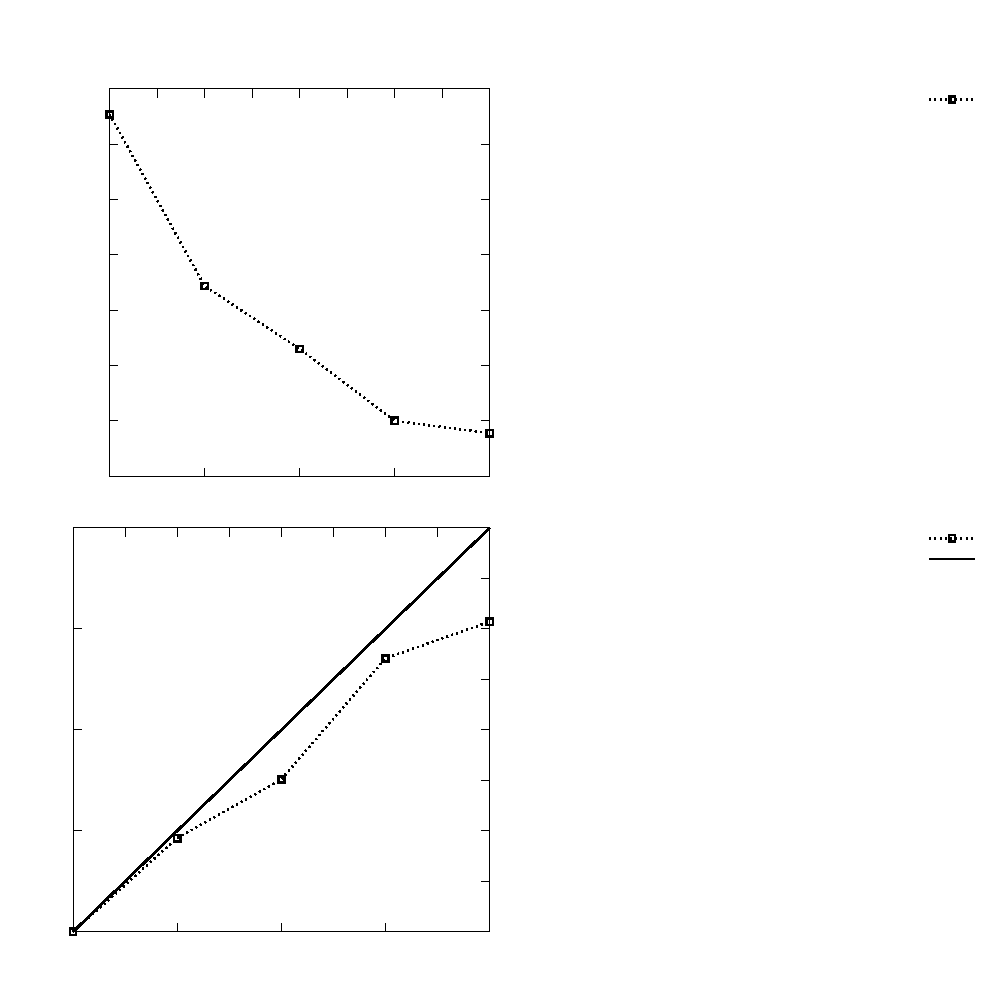
\includegraphics{MPIScalingTimes}}%
    \gplfronttext
  \end{picture}%
\endgroup

	\end{center}
	\caption{
		Solver runtime vs. processors, for polynomial degree $k=1/0$ leading to 212992 DoFs,
		for problem/Equation (\ref{eq:ContantCoeffPoissonBenchmark}).
	}
	\label{fig:Spherek1Time}
\end{figure}

\graphicspath{{./apdx-MPISolverPerformance/strongScaling/NSESphereComplex/plots/}}

\begin{figure}[h!]
	\begin{center}
		% GNUPLOT: LaTeX picture with Postscript
\begingroup
  \makeatletter
  \providecommand\color[2][]{%
    \GenericError{(gnuplot) \space\space\space\@spaces}{%
      Package color not loaded in conjunction with
      terminal option `colourtext'%
    }{See the gnuplot documentation for explanation.%
    }{Either use 'blacktext' in gnuplot or load the package
      color.sty in LaTeX.}%
    \renewcommand\color[2][]{}%
  }%
  \providecommand\includegraphics[2][]{%
    \GenericError{(gnuplot) \space\space\space\@spaces}{%
      Package graphicx or graphics not loaded%
    }{See the gnuplot documentation for explanation.%
    }{The gnuplot epslatex terminal needs graphicx.sty or graphics.sty.}%
    \renewcommand\includegraphics[2][]{}%
  }%
  \providecommand\rotatebox[2]{#2}%
  \@ifundefined{ifGPcolor}{%
    \newif\ifGPcolor
    \GPcolortrue
  }{}%
  \@ifundefined{ifGPblacktext}{%
    \newif\ifGPblacktext
    \GPblacktexttrue
  }{}%
  % define a \g@addto@macro without @ in the name:
  \let\gplgaddtomacro\g@addto@macro
  % define empty templates for all commands taking text:
  \gdef\gplbacktext{}%
  \gdef\gplfronttext{}%
  \makeatother
  \ifGPblacktext
    % no textcolor at all
    \def\colorrgb#1{}%
    \def\colorgray#1{}%
  \else
    % gray or color?
    \ifGPcolor
      \def\colorrgb#1{\color[rgb]{#1}}%
      \def\colorgray#1{\color[gray]{#1}}%
      \expandafter\def\csname LTw\endcsname{\color{white}}%
      \expandafter\def\csname LTb\endcsname{\color{black}}%
      \expandafter\def\csname LTa\endcsname{\color{black}}%
      \expandafter\def\csname LT0\endcsname{\color[rgb]{1,0,0}}%
      \expandafter\def\csname LT1\endcsname{\color[rgb]{0,1,0}}%
      \expandafter\def\csname LT2\endcsname{\color[rgb]{0,0,1}}%
      \expandafter\def\csname LT3\endcsname{\color[rgb]{1,0,1}}%
      \expandafter\def\csname LT4\endcsname{\color[rgb]{0,1,1}}%
      \expandafter\def\csname LT5\endcsname{\color[rgb]{1,1,0}}%
      \expandafter\def\csname LT6\endcsname{\color[rgb]{0,0,0}}%
      \expandafter\def\csname LT7\endcsname{\color[rgb]{1,0.3,0}}%
      \expandafter\def\csname LT8\endcsname{\color[rgb]{0.5,0.5,0.5}}%
    \else
      % gray
      \def\colorrgb#1{\color{black}}%
      \def\colorgray#1{\color[gray]{#1}}%
      \expandafter\def\csname LTw\endcsname{\color{white}}%
      \expandafter\def\csname LTb\endcsname{\color{black}}%
      \expandafter\def\csname LTa\endcsname{\color{black}}%
      \expandafter\def\csname LT0\endcsname{\color{black}}%
      \expandafter\def\csname LT1\endcsname{\color{black}}%
      \expandafter\def\csname LT2\endcsname{\color{black}}%
      \expandafter\def\csname LT3\endcsname{\color{black}}%
      \expandafter\def\csname LT4\endcsname{\color{black}}%
      \expandafter\def\csname LT5\endcsname{\color{black}}%
      \expandafter\def\csname LT6\endcsname{\color{black}}%
      \expandafter\def\csname LT7\endcsname{\color{black}}%
      \expandafter\def\csname LT8\endcsname{\color{black}}%
    \fi
  \fi
    \setlength{\unitlength}{0.0500bp}%
    \ifx\gptboxheight\undefined%
      \newlength{\gptboxheight}%
      \newlength{\gptboxwidth}%
      \newsavebox{\gptboxtext}%
    \fi%
    \setlength{\fboxrule}{0.5pt}%
    \setlength{\fboxsep}{1pt}%
\begin{picture}(9620.00,9620.00)%
    \gplgaddtomacro\gplbacktext{%
      \csname LTb\endcsname%
      \put(938,5037){\makebox(0,0)[r]{\strut{}$0$}}%
      \csname LTb\endcsname%
      \put(938,5673){\makebox(0,0)[r]{\strut{}$10000$}}%
      \csname LTb\endcsname%
      \put(938,6310){\makebox(0,0)[r]{\strut{}$20000$}}%
      \csname LTb\endcsname%
      \put(938,6946){\makebox(0,0)[r]{\strut{}$30000$}}%
      \csname LTb\endcsname%
      \put(938,7582){\makebox(0,0)[r]{\strut{}$40000$}}%
      \csname LTb\endcsname%
      \put(938,8219){\makebox(0,0)[r]{\strut{}$50000$}}%
      \csname LTb\endcsname%
      \put(938,8855){\makebox(0,0)[r]{\strut{}$60000$}}%
      \csname LTb\endcsname%
      \put(1502,4858){\makebox(0,0){\strut{}$10$}}%
      \csname LTb\endcsname%
      \put(2015,4858){\makebox(0,0){\strut{}$20$}}%
      \csname LTb\endcsname%
      \put(2529,4858){\makebox(0,0){\strut{}$30$}}%
      \csname LTb\endcsname%
      \put(3042,4858){\makebox(0,0){\strut{}$40$}}%
      \csname LTb\endcsname%
      \put(3555,4858){\makebox(0,0){\strut{}$50$}}%
      \csname LTb\endcsname%
      \put(4069,4858){\makebox(0,0){\strut{}$60$}}%
      \csname LTb\endcsname%
      \put(4376,5037){\makebox(0,0)[l]{\strut{} }}%
      \csname LTb\endcsname%
      \put(4376,5673){\makebox(0,0)[l]{\strut{} }}%
      \csname LTb\endcsname%
      \put(4376,6310){\makebox(0,0)[l]{\strut{} }}%
      \csname LTb\endcsname%
      \put(4376,6946){\makebox(0,0)[l]{\strut{} }}%
      \csname LTb\endcsname%
      \put(4376,7582){\makebox(0,0)[l]{\strut{} }}%
      \csname LTb\endcsname%
      \put(4376,8219){\makebox(0,0)[l]{\strut{} }}%
      \csname LTb\endcsname%
      \put(4376,8855){\makebox(0,0)[l]{\strut{} }}%
      \csname LTb\endcsname%
      \put(1040,9034){\makebox(0,0){\strut{} }}%
      \csname LTb\endcsname%
      \put(1502,9034){\makebox(0,0){\strut{} }}%
      \csname LTb\endcsname%
      \put(1964,9034){\makebox(0,0){\strut{} }}%
      \csname LTb\endcsname%
      \put(2426,9034){\makebox(0,0){\strut{} }}%
      \csname LTb\endcsname%
      \put(2888,9034){\makebox(0,0){\strut{} }}%
      \csname LTb\endcsname%
      \put(3350,9034){\makebox(0,0){\strut{} }}%
      \csname LTb\endcsname%
      \put(3812,9034){\makebox(0,0){\strut{} }}%
      \csname LTb\endcsname%
      \put(4274,9034){\makebox(0,0){\strut{} }}%
    }%
    \gplgaddtomacro\gplfronttext{%
      \csname LTb\endcsname%
      \put(236,6946){\rotatebox{-270}{\makebox(0,0){\strut{}Time [s]}}}%
      \csname LTb\endcsname%
      \put(4668,6946){\rotatebox{-270}{\makebox(0,0){\strut{}SlvIter}}}%
      \csname LTb\endcsname%
      \put(2657,9482){\makebox(0,0){\strut{}Exclusive times}}%
      \csname LTb\endcsname%
      \put(8737,8765){\makebox(0,0)[r]{\strut{}Swz w Coarse MGLevels2}}%
      \csname LTb\endcsname%
      \put(8737,8586){\makebox(0,0)[r]{\strut{}Swz Kcycle w Coarse Overlap MGLevels2}}%
      \csname LTb\endcsname%
      \put(8737,8407){\makebox(0,0)[r]{\strut{}Swz w Coarse Overlap MGLevels2}}%
    }%
    \gplgaddtomacro\gplbacktext{%
      \csname LTb\endcsname%
      \put(632,620){\makebox(0,0)[r]{\strut{}$0$}}%
      \csname LTb\endcsname%
      \put(632,1115){\makebox(0,0)[r]{\strut{}$5$}}%
      \csname LTb\endcsname%
      \put(632,1610){\makebox(0,0)[r]{\strut{}$10$}}%
      \csname LTb\endcsname%
      \put(632,2106){\makebox(0,0)[r]{\strut{}$15$}}%
      \csname LTb\endcsname%
      \put(632,2601){\makebox(0,0)[r]{\strut{}$20$}}%
      \csname LTb\endcsname%
      \put(632,3096){\makebox(0,0)[r]{\strut{}$25$}}%
      \csname LTb\endcsname%
      \put(632,3591){\makebox(0,0)[r]{\strut{}$30$}}%
      \csname LTb\endcsname%
      \put(632,4087){\makebox(0,0)[r]{\strut{}$35$}}%
      \csname LTb\endcsname%
      \put(632,4582){\makebox(0,0)[r]{\strut{}$40$}}%
      \csname LTb\endcsname%
      \put(1240,441){\makebox(0,0){\strut{}$10$}}%
      \csname LTb\endcsname%
      \put(1802,441){\makebox(0,0){\strut{}$20$}}%
      \csname LTb\endcsname%
      \put(2364,441){\makebox(0,0){\strut{}$30$}}%
      \csname LTb\endcsname%
      \put(2925,441){\makebox(0,0){\strut{}$40$}}%
      \csname LTb\endcsname%
      \put(3487,441){\makebox(0,0){\strut{}$50$}}%
      \csname LTb\endcsname%
      \put(4049,441){\makebox(0,0){\strut{}$60$}}%
      \csname LTb\endcsname%
      \put(4376,620){\makebox(0,0)[l]{\strut{} }}%
      \csname LTb\endcsname%
      \put(4376,1115){\makebox(0,0)[l]{\strut{} }}%
      \csname LTb\endcsname%
      \put(4376,1610){\makebox(0,0)[l]{\strut{} }}%
      \csname LTb\endcsname%
      \put(4376,2106){\makebox(0,0)[l]{\strut{} }}%
      \csname LTb\endcsname%
      \put(4376,2601){\makebox(0,0)[l]{\strut{} }}%
      \csname LTb\endcsname%
      \put(4376,3096){\makebox(0,0)[l]{\strut{} }}%
      \csname LTb\endcsname%
      \put(4376,3591){\makebox(0,0)[l]{\strut{} }}%
      \csname LTb\endcsname%
      \put(4376,4087){\makebox(0,0)[l]{\strut{} }}%
      \csname LTb\endcsname%
      \put(4376,4582){\makebox(0,0)[l]{\strut{} }}%
      \csname LTb\endcsname%
      \put(734,4761){\makebox(0,0){\strut{} }}%
      \csname LTb\endcsname%
      \put(1240,4761){\makebox(0,0){\strut{} }}%
      \csname LTb\endcsname%
      \put(1745,4761){\makebox(0,0){\strut{} }}%
      \csname LTb\endcsname%
      \put(2251,4761){\makebox(0,0){\strut{} }}%
      \csname LTb\endcsname%
      \put(2757,4761){\makebox(0,0){\strut{} }}%
      \csname LTb\endcsname%
      \put(3263,4761){\makebox(0,0){\strut{} }}%
      \csname LTb\endcsname%
      \put(3768,4761){\makebox(0,0){\strut{} }}%
      \csname LTb\endcsname%
      \put(4274,4761){\makebox(0,0){\strut{} }}%
    }%
    \gplgaddtomacro\gplfronttext{%
      \csname LTb\endcsname%
      \put(236,2601){\rotatebox{-270}{\makebox(0,0){\strut{}Time [s]}}}%
      \csname LTb\endcsname%
      \put(4668,2601){\rotatebox{-270}{\makebox(0,0){\strut{}SlvInit}}}%
      \csname LTb\endcsname%
      \put(2504,173){\makebox(0,0){\strut{}Processors}}%
      \csname LTb\endcsname%
      \put(8737,4492){\makebox(0,0)[r]{\strut{}Swz w Coarse MGLevels2}}%
      \csname LTb\endcsname%
      \put(8737,4313){\makebox(0,0)[r]{\strut{}Swz Kcycle w Coarse Overlap MGLevels2}}%
      \csname LTb\endcsname%
      \put(8737,4134){\makebox(0,0)[r]{\strut{}Swz w Coarse Overlap MGLevels2}}%
    }%
    \gplbacktext
    \put(0,0){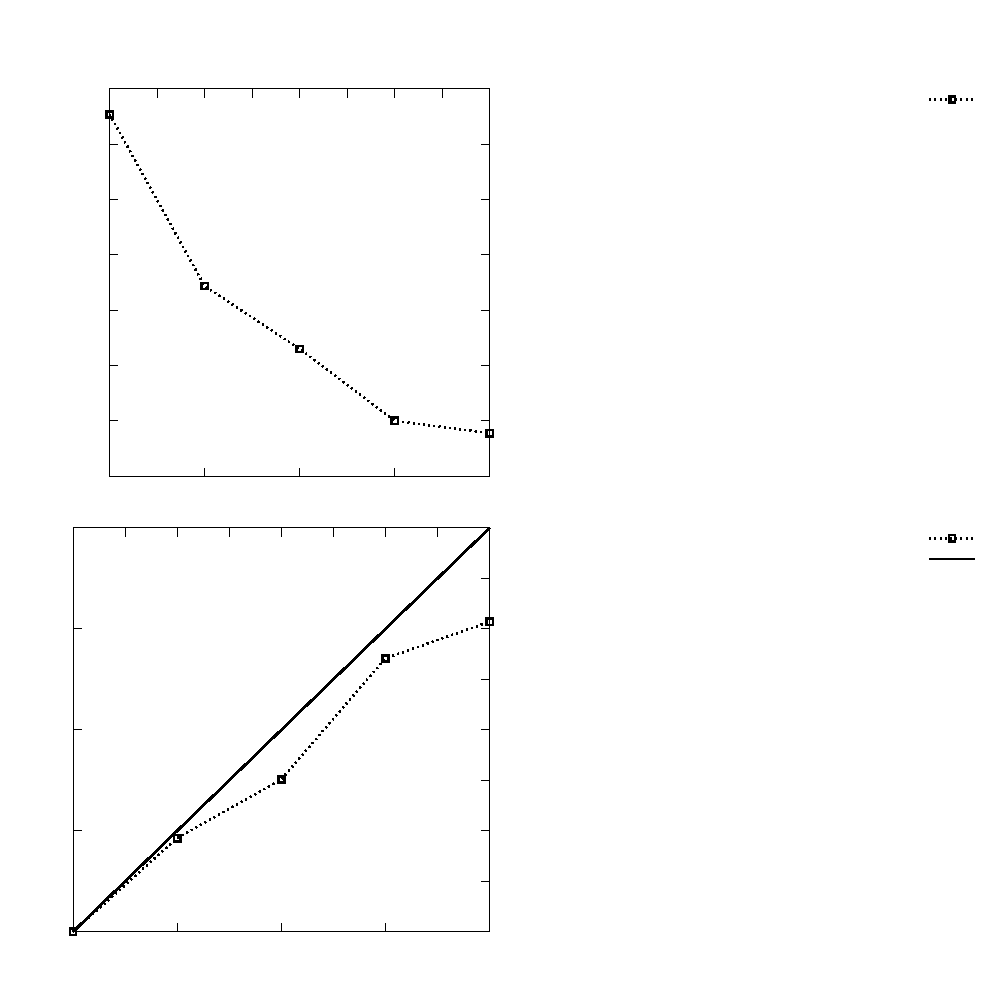
\includegraphics{MPIScalingTimes}}%
    \gplfronttext
  \end{picture}%
\endgroup

	\end{center}
	\caption{
		Solver runtime vs. processors, for polynomial degree $k=2/1$ leading to 557056 DoFs,
		for problem/Equation (\ref{eq:ContantCoeffPoissonBenchmark}).
	}
	\label{fig:Spherek1Time}
\end{figure}